\documentclass{beamer}

\usepackage{beamerthemesplit}
\usepackage[brazil]{babel}
\usepackage[utf8]{inputenc}
\usepackage{pdfanim}

\usepackage{graphicx}
\usepackage{picinpar}

\usepackage{graphics}
\usepackage{wrapfig}
\usepackage{floatfig}

\PDFAnimLoad[width=0.5\linewidth,auto,loop,remember]{dijkstra}{animacoes/dijkstra}{54}

\setbeamertemplate{footline}
{%
\leavevmode%
\hbox{%

\begin{beamercolorbox}[wd=.5\paperwidth,ht=2.5ex,dp=1.125ex,right]{author
in head/foot}%
\usebeamerfont{title in head/foot}\insertshortauthor\hspace{.3cm}
\end{beamercolorbox}%

\begin{beamercolorbox}[wd=.46\paperwidth,ht=2.5ex,dp=1.125ex,left]{title
in head/foot}%
\usebeamerfont{author in head/foot}\hspace{.3cm}\insertshorttitle
\end{beamercolorbox}%

\begin{beamercolorbox}[wd=.04\paperwidth,ht=2.5ex,dp=1.125ex,center]{title
in head/foot}%
\usebeamerfont{author in
head/foot}\insertframenumber/\inserttotalframenumber
\end{beamercolorbox}%
}%
\vskip0pt%
}%\setbeamertemplate{navigation symbols}{}
%\setbeamertemplate
%{footline}
%{\quad\strut\insertsection
%\hfill\insertframenumber/\inserttotalframenumber\strut\quad} 

\title{Navegação e Monitoramento de Ambientes Internos Utilizando Robôs Móveis}
\author{Heitor L. Polidoro}
\date{\today}

\begin{document}
\section{Contruindo}
%\frame{\titlepage}
%
%\section[Roteiro]{}
%\frame{\tableofcontents}
%
%\section{Introdução}
%\subsection{Robótica Móvel}
%\frame
%{
%  \begin{itemize}
%  \item Problemas da robótica móvel.
%		\begin{itemize}
%			\item Navegação, Exploração, etc.
%		\end{itemize}
%	\item Projeto
%		\begin{itemize}
%			\item Monitoramento de ambientes internos
%		\end{itemize}
%  \end{itemize}
%}
%
%\section{Projeto}
%\subsection{Visão Geral}
%\frame
%{
%\begin{itemize}
%	\item Desvio de obstáculos
%		\begin{itemize}
%			\item Campos Potenciais
%		\end{itemize}
%	\item Busca do menos caminho
%		\begin{itemize}
%			\item Dijkstra
%		\end{itemize}
%	\item Controle do Robô
%		\begin{itemize}
%			\item Player/Stage
%		\end{itemize}
%	\item Definição da tragetória
%		
%		
%
%\end{itemize}
%}
%
%\subsection{Campos Potenciais}
%\frame
%{
%	\frametitle{Definição}
%       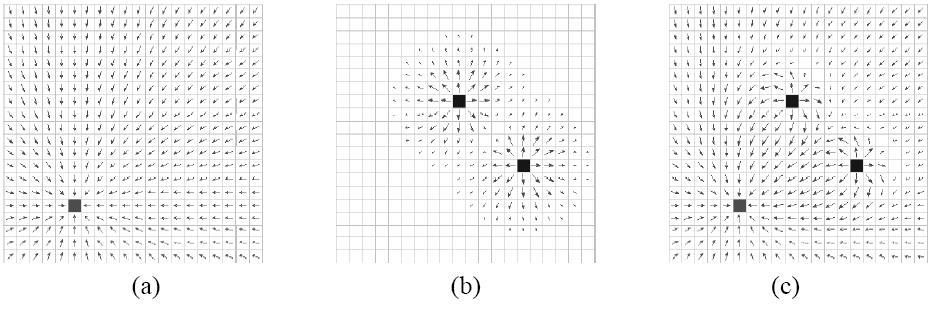
\includegraphics[width=1\linewidth]{imagens/cp_combinacao.jpg}
%		\\
%	 a) Meta\\
%	 b) Obstáculos\\
%	 c) Combinação
%}
%
%\frame
%{
%	\frametitle{Mínimos Locais}
%      \centering
%       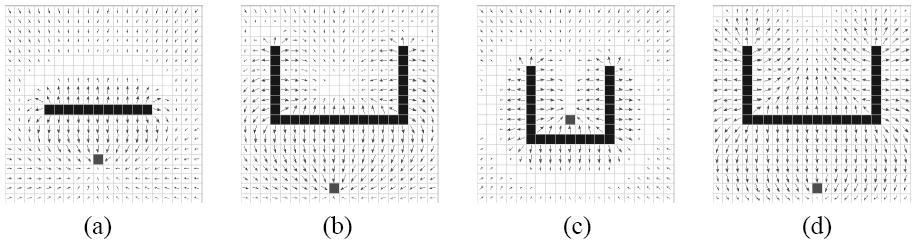
\includegraphics[width=1\linewidth]{imagens/cp_minimos_locais.jpg}
%}
%	
%\frame
%{
%	\frametitle{Implementação}
%	\begin{wrapfigure}[3]{r}{5cm}  % [nºde linhas que a figura vai ocupar]{posição - l, r, c}{largura da figura - Xcm}
%		       \centering  % figura centralizada
%	  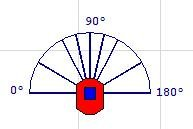
\includegraphics[width=5cm]{imagens/laser.jpg}
%   \end{wrapfigure}
%$ $
%	\begin{itemize}
%		\item 9 ângulos 
%			\begin{itemize}
%				\item	($0^{\circ},\,30^{\circ},\,60^{\circ},\,75^{\circ},\,90^{\circ},$\\$105^{\circ},\,120^{\circ},\,150^{\circ},\,180$)
%			\end{itemize}
%		\item Distância máxima conciderada: 1 m
%		\item Distância mínima de segurança: 0,6 m
%			\begin{itemize}
%				\item Somente noa ângulos $60^{\circ},\,75^{\circ},\,90^{\circ},\,105^{\circ},\,120^{\circ}$
%			\end{itemize}
%		\item Velocidades
%			\begin{itemize}
%				\item Linear: 0,25 m/s e 0,375 m/s
%				\item Rotação: 0,5 rad/s e 0,1 rad/s
%			\end{itemize}
%	\end{itemize}
%}
%
%\subsection{Dijkstra}
%\frame{
%%  \begin{center}
%%		\begin{tabular}{|c|c|}
%%			\hline
%%			\begin{minipage}{4cm}
%%				\begin{itemize}
%%					\item Menor caminho da origem até todos os vértices
%%					\item Contrução do caminho ao vertice desejado
%%				\end{itemize}
%%		\end{minipage}
%%		& 
%%
%%%		blablabla\\
%%%	  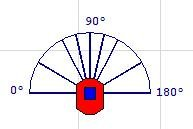
\includegraphics[width=5cm]{imagens/laser.jpg}\\
%%		\PDFAnimation{dijkstra} \\
%%			\hline
%%  \end{tabular}
%%  \end{center}
%%
%	\begin{itemize}
%		\item Menor caminho da origem até todos os vértices
%		\item ``Monto'' o caminho ao vertice desejado
%	\end{itemize}
%	\begin{center}
%		\PDFAnimation{dijkstra}
%	\end{center}
%}
%
%\subsection{Controle do Robô}
%\frame
%{
%\begin{itemize}
%	\item Player
%		\begin{itemize}
%			\item O robô é um servidor;
%			\item Clientem em: C, \underline{C++}, Java, Python;
%			\item Sockets TCP.
%		\end{itemize}
%	\item Stage
%		\begin{itemize}
%			\item Simulador.
%		\end{itemize}
%\end{itemize}
%}

\frame{
\begin{itemize}
	\item Stage
		\begin{itemize}
			\item Simulação com 6 robôs, 2 objetos, laser, sonar e blobfinder.
		\end{itemize}
\end{itemize}
\begin{center}
	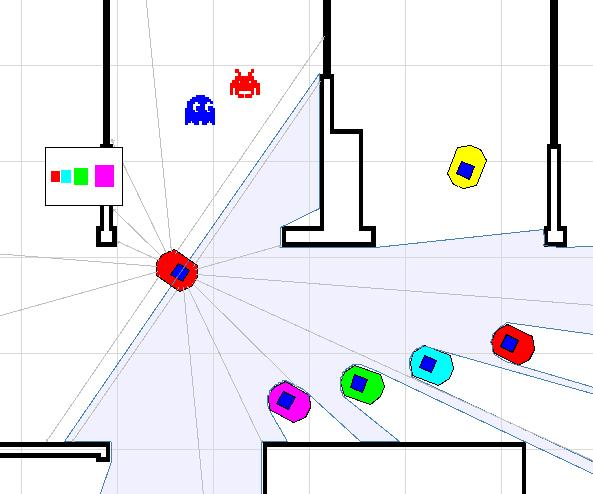
\includegraphics[width=5cm]{imagens/stage.jpg}
\end{center}
}

\end{document}
